\documentclass{article}

\usepackage{enumerate}
\usepackage{amsmath}
\usepackage{amssymb}
\usepackage{amsfonts}
\usepackage{mathtools}
\usepackage{graphicx}
\usepackage{float}
\usepackage{caption}
\usepackage{subcaption}
\usepackage{color}
\usepackage{relsize}
\usepackage{algpseudocode}
\usepackage[procnames]{listings}
\usepackage[colorlinks = true, allcolors = blue]{hyperref}
\usepackage[]{units}
\usepackage{framed}
\usepackage{breqn}
\usepackage{lipsum}
\usepackage{algorithm}
\usepackage{algpseudocode}
\usepackage{fancyhdr}
\usepackage{extramarks}
\usepackage{xfrac}
\usepackage{multicol}
\usepackage{bibentry}
\usepackage{verbatim}
\nobibliography*

\def\arraystretch{1.2}

\topmargin = -0.45in
\evensidemargin = 0in
\oddsidemargin = 0in
\textwidth = 6.5in
\textheight = 9.0in
\headsep = 0.25in

\pagestyle{fancy}
\lhead{Pedro D. Bello-Maldonado}
\chead{}
\rhead{Research notes}
\lfoot{IBM Research - Sustainability}
\cfoot{\thepage}
\rfoot{\today}

\renewcommand\headrulewidth{0.4pt}
\renewcommand\footrulewidth{0.4pt}

\renewcommand{\algorithmicrequire}{\textbf{Input:}}
\renewcommand{\algorithmicensure}{\textbf{Output:}}
\renewcommand{\algorithmicforall}{\textbf{parallel for}}

\setlength{\parindent}{0pt}
\setlength{\parskip}{5pt plus 1pt minus 1pt}

\begin{document}
    \section*{Sustainability}
    {
        \textbf{Objective:} Reduce the carbon footprint of computing applications

        \subsection*{Ideas}
        {
            \begin{itemize}
                \item Define application specific standards for data packing so serving is as efficient as possible

                    \begin{itemize}
                        \item A lot of data reading and serving tools (e.g., databases, file formats, etc.) aim to be general purpose in order to increase the number of users. This approach misses the opportunity to optimize data accessing for applications that don't need the full set of features available in these tools.
                        \item From the Facebook AI sustainability paper: ``... application-level caching improves power efficiency by 6.7$\times$".
                    \end{itemize}

                \item Control the allocation of resources so that strong scaling is fixed at the strong-scale limit\footnotemark, thus minimizing the overhead impact of distributed computing infrastructure management
                    \footnotetext{\textit{Strong-scale limit:} Scaling point at which adding more processors doesn't reduce the execution time in the same proportion.}

                    \begin{itemize}
                        \item Strong scaling allows an application to add more computing resources that proportionally reduce the execution time. The parallelization of the application adds some overhead which in turns affects the total potential speedup. In many cases this cannot be avoided, and so limitting the number of resources given to the system can reduce the power consumption of the application that goes into overhead.
                        \item On a different direction, add as many computing resources as needed so the execution time and power consumption are minimized.
                    \end{itemize}

                    \begin{figure}[!h]
                        \centering
                        \begin{subfigure}[b]{0.45 \textwidth}
                            \centering
                            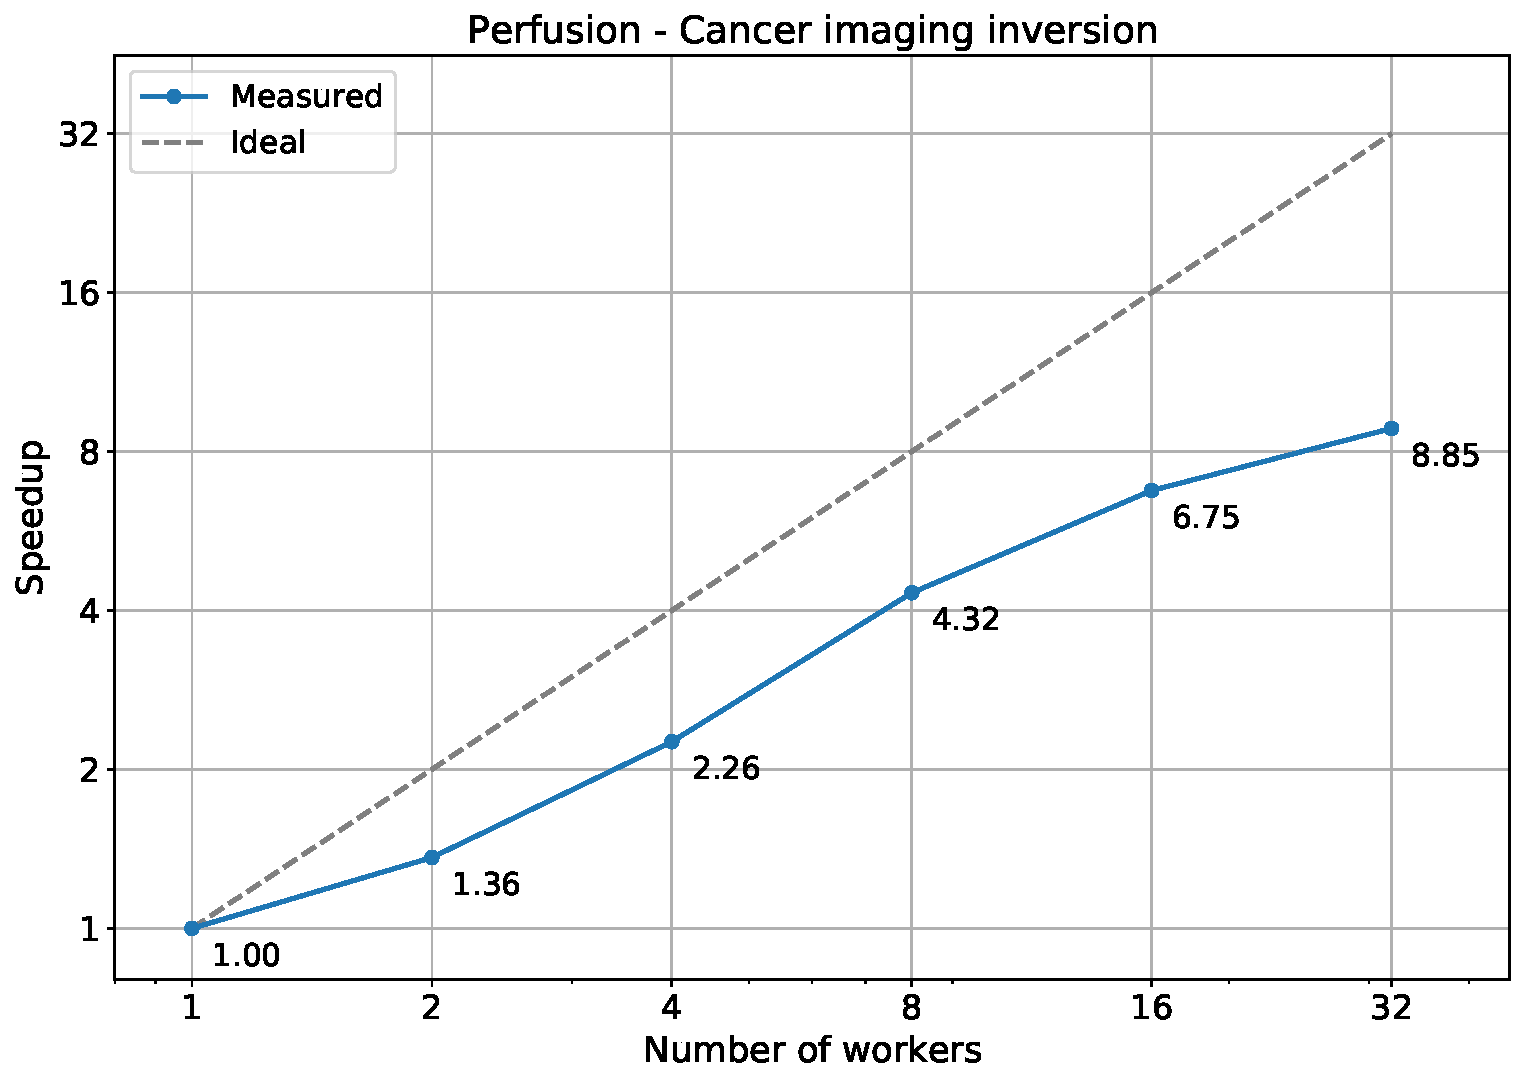
\includegraphics[width = 1.0 \textwidth]{Figures/perfusion.pdf}
                            \caption{Application A}
                        \end{subfigure}
                        \begin{subfigure}[b]{0.45 \textwidth}
                            \centering
                            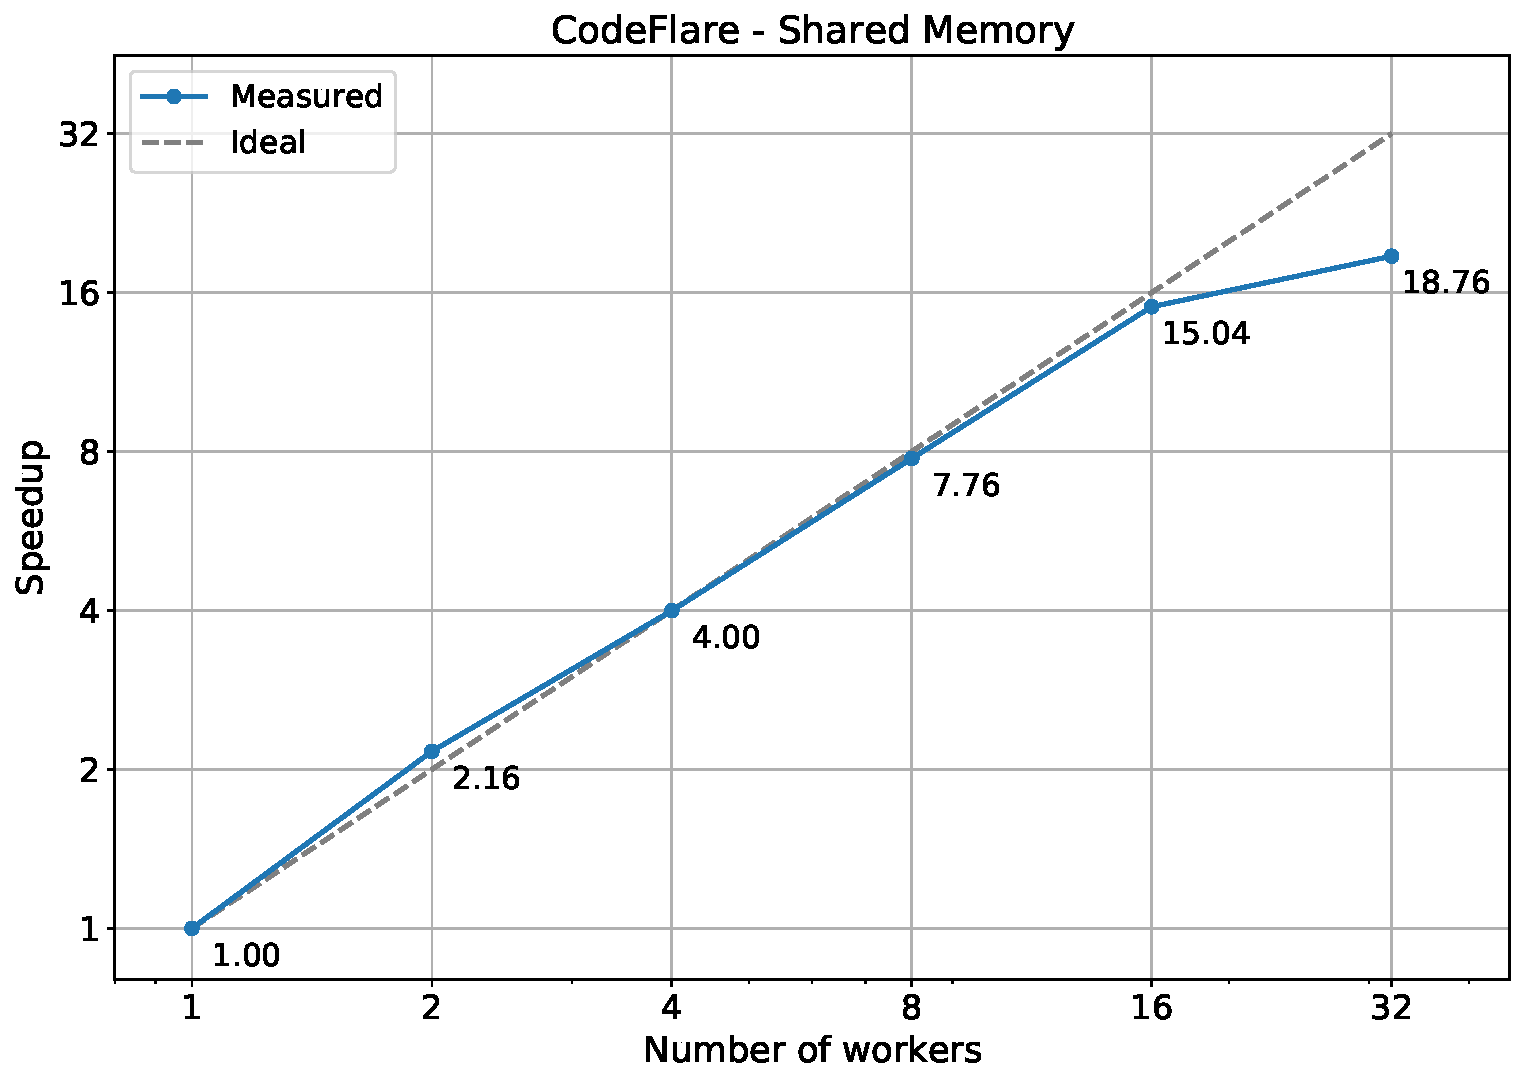
\includegraphics[width = 1.0 \textwidth]{Figures/codeflare.pdf}
                            \caption{Application B}
                        \end{subfigure}
                        \caption{Strong scaling of two \textbf{very} different applications exhibiting different performance. Application B strong scales well up to 16 processors while Aplication A is not using the resources efficiently resulting in bad scaling.}
                    \end{figure}

                \item Load distribution accross centers operating in different time zones (some data-centers won't be fully utilized at night)
            \end{itemize}
        }
    }
\end{document}
